\section{Knowledge Graphs}
\begin{quote}
    “A knowledge graph consists of a set of
interconnected typed entities and their
attributes."
\end{quote}
Nella rappresentazione e nel ragionamento della conoscenza, il knowledge graph è una base di conoscenza che utilizza un modello di dati o una topologia strutturata a grafo per integrare i dati. I knowledge graph sono spesso utilizzati per memorizzare descrizioni interconnesse di entità, oggetti, eventi, situazioni o concetti astratti, codificando anche la semantica sottostante la terminologia utilizzata. Sono ampiamente associati e utilizzati da motori di ricerca come Google, motori di conoscenza e servizi di domande e risposte come WolframAlpha, Siri di Apple e Amazon Alexa; e social network come LinkedIn e Facebook.
Rispetto ad altri sistemi informativi orientati alla conoscenza, i knowledge graph si distinguono per la loro particolare combinazione di: 
\begin{itemize}
    \item Strutture di rappresentazione della conoscenza e ragionamento, come linguaggi, schemi, vocabolari standard e gerarchie tra concetti; 
    \item Processi di gestione delle informazioni (come le informazioni vengono assimilate e trasformate in un knowledge graph);
    \item Modelli di accesso ed elaborazione, come meccanismi di interrogazione, algoritmi di ricerca e tecniche di pre e post-elaborazione.
\end{itemize}

\paragraph{Definizione} Un knowledge graph é un grafo costituito da concetti, classi, proprietà, relazioni e descrizioni di entità. I dati possono essere aperti, privati o chiusi; possono inoltre essere originali, derivati o aggregati. 
\\
I knowledge graphs vengono generalmente rappresentati tramite l'utilizzo di Resource Description Frameworks (RDF). La struttura sottostante di qualsiasi espressione in RDF è una raccolta di triple, ciascuna composta da un soggetto, un predicato e un oggetto. Ogni tripla può essere rappresentata come un collegamento nodo-arco-nodo, chiamato anche grafo RDF.
\\
\begin{figure}[th]
    \centering
    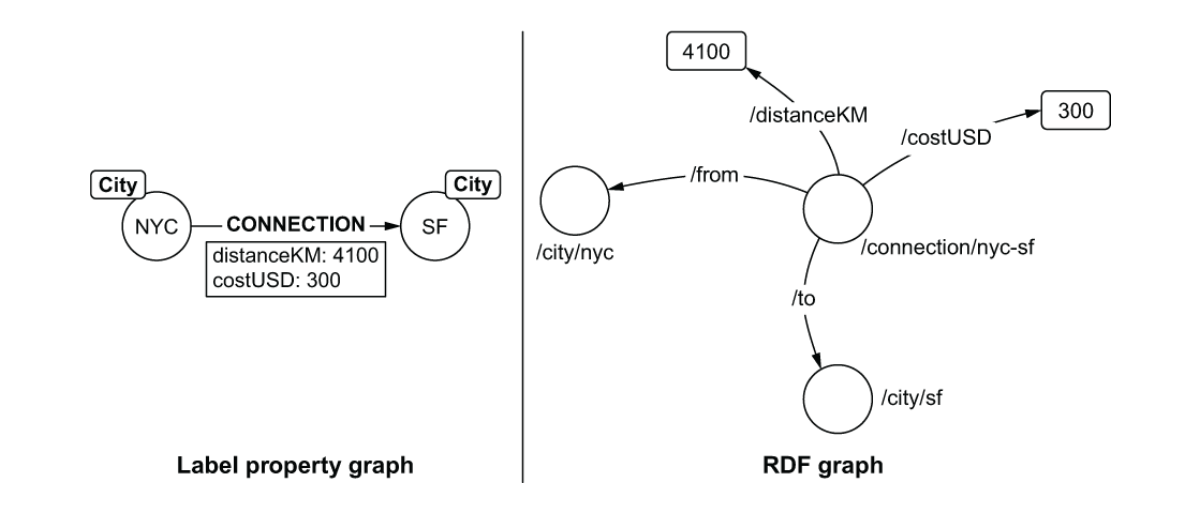
\includegraphics[width=0.8\linewidth]{KnowledgeGraphs//img/labelvsrdf.png}
\end{figure}
\\
Un Knowledge Graph è un insieme di dati ed è:
\begin{itemize}
    \item \textbf{Strutturato} (sotto forma di una specifica struttura dati)
    \item \textbf{Normalizzato} (costituito da piccole unità, come vertici e archi)
    \item \textbf{Connesso} (definito dalle connessioni - anche distanti (non dirette) - tra gli oggetti)
\end{itemize}
Inoltre, i Knowledge Graph sono in genere:
\begin{itemize}
    \item \textbf{Espliciti} (creati appositamente con un significato specifico)
    \item \textbf{Dichiarativi} (significativi di per sé, indipendenti da una particolare implementazione o algoritmo)
    \item \textbf{Annotati} (arricchiti con informazioni contestuali per registrare ulteriori dettagli e metadati)
    \item \textbf{Non gerarchici} (più di una semplice struttura ad albero)
    \item \textbf{Grandi dimensioni} (milioni anziché centinaia di elementi)
\end{itemize}

\subsection{Creating Knowledge Graphs}
La creazione di \textit{knowledge graphs} (KG) può essere affrontata attraverso diversi approcci, che si distinguono per livello di automazione, qualità, e scalabilità. Di seguito vengono descritti i principali paradigmi.

\vspace{1em}
\textbf{1. Approcci curati (\textit{Curated approaches})}
\begin{itemize}
  \item I \textbf{tripli} (soggetto, predicato, oggetto) vengono creati manualmente da un gruppo chiuso di esperti.
  \item Tali approcci sono \textbf{altamente accurati}, grazie all'intervento umano esperto.
  \item Tuttavia, \textbf{non sono scalabili} a causa dell'alto costo e tempo richiesto.
  \item \textbf{Esempi} noti:
  \begin{itemize}
    \item \textit{Cyc/OpenCyc}
    \item \textit{WordNet}
    \item \textit{UMLS} (Unified Medical Language System)
    \item \textit{SNOMED CT} (Systematized Nomenclature of Medicine Clinical Terms)
  \end{itemize}
\end{itemize}

\vspace{1em}
\textbf{2. Approcci collaborativi (\textit{Collaborative approaches})}
\begin{itemize}
  \item I tripli vengono creati manualmente da una comunità aperta di volontari.
  \item Questi approcci \textbf{scalano meglio} rispetto a quelli curati, grazie al contributo distribuito.
  \item \textbf{Esempi}:
  \begin{itemize}
    \item \textit{Wikidata}
    \item \textit{Freebase}
  \end{itemize}
  \item \textbf{Criticità}:
  \begin{itemize}
    \item \textit{Incompletezza}: ad esempio, il 71\% delle persone in Freebase manca del luogo di nascita obbligatorio.
    \item \textit{Crescita rallentata}: sia Wikipedia che Wikidata mostrano un tasso di crescita decrescente.
  \end{itemize}
\end{itemize}

\vspace{1em}
\textbf{3. Approcci automatici da testo semi-strutturato (\textit{Automated semi-structured approaches})}
\begin{itemize}
  \item I tripli vengono estratti automaticamente da testi semi-strutturati tramite:
  \begin{itemize}
    \item Regole scritte manualmente
    \item Regole apprese automaticamente
    \item Espressioni regolari
  \end{itemize}
  \item Si sfruttano fonti come le \textbf{infobox di Wikipedia}, che offrono dati strutturati in modo parziale.
  \item Questi approcci offrono un buon \textbf{compromesso tra accuratezza e scalabilità}.
  \item \textbf{Esempi}:
  \begin{itemize}
    \item \textit{YAGO}
    \item \textit{DBpedia}
    \item \textit{Freebase}
  \end{itemize}
  \item \textbf{Accuratezza} stimata:
  \begin{itemize}
    \item \textit{YAGO2}: oltre il 95\% (verifica manuale)
    \item \textit{Freebase}: circa il 99\%
  \end{itemize}
  \item \textbf{Limiti}: coprono solo una piccola parte delle informazioni presenti sul Web.
\end{itemize}

\vspace{1em}
\textbf{4. Approcci automatici da testo non strutturato (\textit{Automated unstructured approaches})}
\begin{itemize}
  \item I tripli sono estratti automaticamente da testo \textbf{non strutturato}, come pagine Web o articoli.
  \item Si utilizzano tecniche di \textbf{machine learning} e \textbf{natural language processing (NLP)}.
  \item I sistemi imparano a identificare entità, relazioni e concetti direttamente da testi in linguaggio naturale.
  \item \textbf{Esempi} di sistemi:
  \begin{itemize}
    \item \textit{NELL} (Never-Ending Language Learning)
    \item \textit{Knowledge Vault}
    \item \textit{PATTY}, \textit{PROSPERA}
    \item \textit{DeepDive}, \textit{Elementary}
    \item \textit{ReVerb}, \textit{OLLIE}, \textit{PRISMATIC}
  \end{itemize}
  \item \textbf{Sfide}:
  \begin{itemize}
    \item Presenza di \textbf{rumore} (informazioni errate o imprecise).
    \item La qualità può essere migliorata integrando \textbf{conoscenze da repository esistenti e affidabili}.
  \end{itemize}
\end{itemize}

\vspace{1em}
\textbf{5. Collegamento di dataset esistenti (\textit{Linking existing datasets})}
\begin{itemize}
  \item Diversi dataset vengono interconnessi utilizzando principi di \textbf{linked data}.
  \item Questo approccio arricchisce il grafo di conoscenza, mantenendo coerenza e interoperabilità tra fonti diverse.
\end{itemize}

\subsection{Knowledge Graphs and Important Nodes}

Nei \textit{knowledge graphs}, la determinazione dell'\textbf{importanza dei nodi} non si basa unicamente sulla loro connettività, ma può dipendere da ulteriori elementi semantici e strutturali. In particolare, possono influenzare l'importanza:

\begin{itemize}
  \item Le \textbf{proprietà associate agli archi} (\textit{edge attributes}), che rappresentano il tipo e il significato delle relazioni tra nodi. Ad esempio, un arco \texttt{hasSpouse} può essere considerato più rilevante di un arco \texttt{likesMusicGenre}.
  
  \item Le \textbf{etichette dei nodi} (\textit{node labels}) o altri attributi semantici dei nodi stessi. Queste etichette possono fornire informazioni sul tipo di entità (es. \texttt{Person}, \texttt{Organization}) o sul loro ruolo nel grafo.

  \item La possibilità di \textbf{ignorare nodi o relazioni specifiche} che non aggiungono informazione utile. Ad esempio:
  \begin{itemize}
    \item In un knowledge graph codificato in \textit{OWL} (Web Ontology Language), ogni entità ha una tripla del tipo:
    \begin{center}
      \texttt{:entity rdf:type owl:Thing}
    \end{center}
    \item Poiché questa informazione è condivisa da tutte le entità, può essere considerata \textbf{ridondante} o \textbf{irrilevante} nel calcolo dell'importanza, e quindi ignorata.
  \end{itemize}
\end{itemize}

In sintesi, la valutazione dei nodi più rilevanti in un knowledge graph dovrebbe considerare non solo la struttura topologica, ma anche la semantica implicita nei dati e nei metadati associati.

\subsection{Semantic Similarity}
In un Knowledge Graph, entitá simili sono rappresentate da nodi con connessioni simili; per identificare entitá simili dobbiamo trovare strutture simili. L'idea é trovare gli embedding di nodi in un spazio vettoriale dimensionalmente piú piccolo in modo che vettori simili siano nodi nello stesso embedding. Per farlo:
\begin{itemize}
    \item \textbf{Translational methods:} TransE, TransH, TransR, TransEdge,... che utilizzano funzioni di score distance-based
    \item \textbf{Rotation based methods:} RotatE
    \item \textbf{Graph Convolutional Networks:} R-GCN, TransGCN
    \item \textbf{Walk-based methods:} DeepWalk, RDF2Vec
\end{itemize}

\newpage
\subsubsection*{TransE}
\begin{figure}[th]
    \centering
    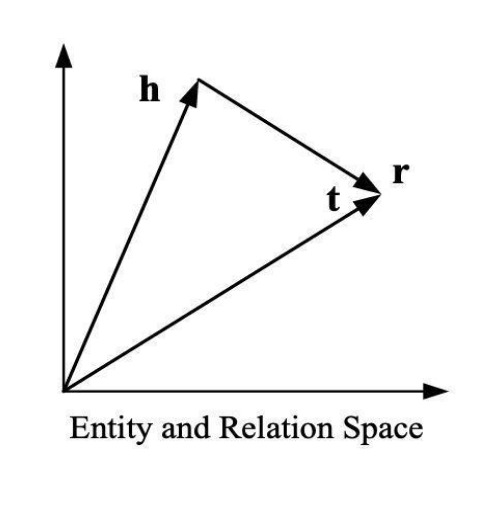
\includegraphics[width=0.4\linewidth]{KnowledgeGraphs//img/transE.png}
\end{figure}
Entitá e relazioni sono mappati nello stesso spazio vettoriale. La relazione $r$ viene considerata una traslazione dalla testa alla coda ma ha problemi con le funzioni simmetriche.
\subsubsection*{TransH}
\begin{figure}[th]
    \centering
    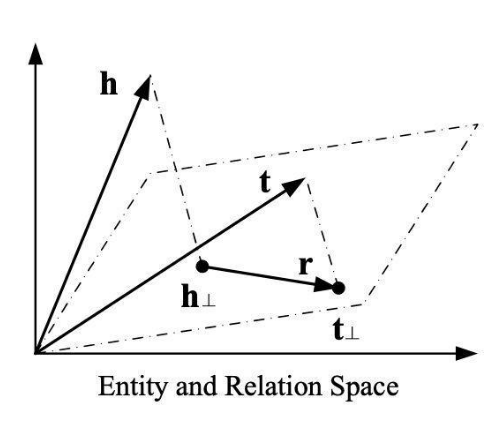
\includegraphics[width=0.4\linewidth]{KnowledgeGraphs//img/transH.png}
\end{figure}
Dallo spazio originale ad un iperpiano, TransH permette diversi ruoli di una entitá all'interno di due relazioni diverse. Le entities $h$ e $t$ vengono proiettate in un iperpiano di relazione $r$. 

\subsection{Knowledge Graph Refinement}
Come modello del mondo reale o di una sua parte, i grafi della conoscenza non possono ragionevolmente raggiungere una copertura completa, ovvero contenere informazioni su ogni singola entità dell'universo. È improbabile, in particolare se si applicano metodi euristici per la costruzione di un grafo della conoscenza, che il grafo della conoscenza sia completamente corretto.
